\chapter{Gestión de Proyectos}

Scrum es un marco de gestión de proyectos para el desarrollo incremental de productos, valiéndose de equipos autoorganizados. 



\subsection{Proyecto Scrum}

Un proyecto, en ingeniería de software, es un esfuerzo temporal que se lleva a cabo para crear un sistema, software o resultado único\footnote{Se parafrasea la definición del PMBOOK \cite{PMBOK-2004}.}. Los proyectos son organizados, en una empresa u organización, por el proceso de administración de proyectos. Según este proceso, el ciclo de vida de los proyectos se puede dividir en tres fases: inicio, ejecución y cierre (ver figura \ref{fig:PMIProject}). En la administración de proyectos es necesario planificar los proyectos y dicha actividad se suele hacer en la fase de inicio ("Starting phase" o "Project Start"). Pero, a diferencia de la metodología clásica (ver figura \ref{fig:PMIProject}) en que la planificación estaba siempre al inicio y el desarrollo en la fase de ejecución, en el marco Scrum la planificación se distribuye durante todo el ciclo de vida del proyecto y en la fase de ejecución se hace el desarrollo incremental de productos (por incrementos de producto) en iteraciones cortas (Sprint) donde cada iteración tiene su respectiva planificación (ver figura \ref{fig:ScrumProject}) y su incremento de producto, en caso de haberlo logrado.

\begin{figure}[h]
  \centering
  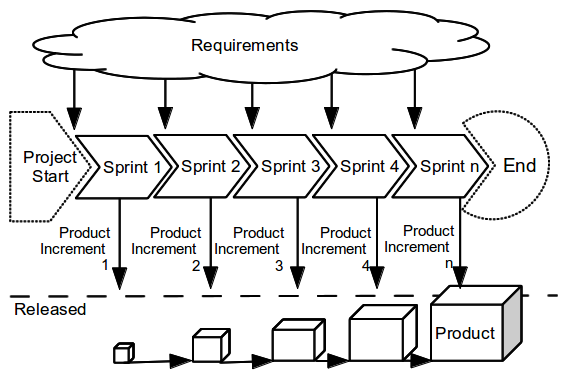
\includegraphics[width=0.90\textwidth]{ScrumProject}
  \caption{Proyecto Scrum}
  \centering
  \label{fig:ScrumProject} %\ref{fig:ScrumProject}
\end{figure}

Entonces podemos decir que en Scrum se piensa en muchos planes periódicos (a corto plazo). Los mismo pueden estar en un plan mayor a largo plazo pero de carácter flexible. También se puede realizar un plan global de entregables en base a los incrementos de producto estimado. Pero, desde esta perspectiva, hay que considerar que aunque se trabaje con planificaciones, los planes no son contratos a respetara a rajatabla.

%Triangle of Project Management
\subsection{Triángulo de la Gestión de proyectos}

El marco de Scrum cambia el triángulo clásico de la gestión de proyectos. El compromiso ya no es entre el tiempo, presupuesto y calidad; sino que se basa en el triángulo de: Presupuesto, Tiempo y funcionalidad (ver figura \ref{fig:ScrumProjectManagementTriangle}).

\begin{figure}[h]
  \centering
  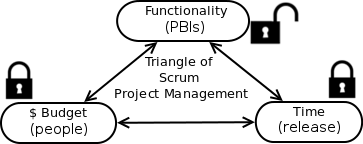
\includegraphics[width=0.80\textwidth]{ScrumProjectManagementTriangle}
  \caption{Triángulo de Gestión de Proyectos Scrum}
  \centering
  \label{fig:ScrumProjectManagementTriangle} %\ref{fig:ScrumProjectManagementTriangle}
\end{figure}

\subsection{Planificación de entregables}

Con esta metodología tampoco es necesario hacer una entrega final (o "releasing") ya que se pueden hacer entregas paulatinas. Para hacer entregas intermedias se puede crear un plan de muy alto nivel para múltiples Sprints durante una planificación de lanzamiento. Este plan de entregables o de de lanzamientos es una guía con la que se pretende reflejar las expectativas sobre las qué funciones se implementarán y cuando se completarán \cite{Scrum-Institute-2015}. También sirve como una base para monitorear el progreso dentro del proyecto. Pero siempre hay que considerar que no es un plan equivalente a un plan clásico, los ítos de releases no deberían ser compromisos rígidos y contractuales, y el desarrollo del proyecto no debería centrarse en respetar el plan. Por este motivo el plan de lanzamiento no es un plan estático. Pues, se cambia durante todo el proyecto cuando nuevos requerimientos o conocimientos están disponible y, por ejemplo, cuando entradas en el Scrum Product Backlog cambian y re-estiman. Por lo tanto este plan debe ser revisado y actualizado en intervalos regulares, por ejemplo, después de cada Sprint.

Para crear un plan de entregables se deben tener disponibles las siguientes cosas:

\begin{enumerate}
\item Un Product Backlog priorizado y estimado.
\item La velocidad estimada del Equipo Scrum.
\item Las condiciones de satisfacción (metas para la agenda, el alcance, los recursos)
\end{enumerate}


